% BOF Preamble
\documentclass[cmpstyle]{ueacmpstyle}
% imports
\usepackage{fancyhdr}
\usepackage{csquotes}
\usepackage{wrapfig}
\usepackage{natbib}
\pagestyle{fancy}
\fancyhead{}
\fancyfoot{}
\lfoot{100036248}
\rfoot{Page \thepage}
\renewcommand{\footrulewidth}{0.4pt}
% macros
% EOF Preamble

% BOF Document
\begin{document}
	\title{Much ado about Everything: \\ The Configuration Management Story}
	\author{Christopher A. Irvine}
	\date{\today}
	\maketitle
	
	\begin{abstract}
	Configuration Management (CM) was created by the U.S. Department of Defence in the mid 1950s to provide a level of consistency in the hardware that was being used by the military. Allowing the training needed to perform maintenance on that hardware to be generalised, reducing costs. For the next 40 years, CM was refined into a distinct technical disciple and was picked up by private industries, eventually enforced by newly created Standard Developing Organisations. 
	
	Today, CM is considered a staple in the administration and management of large projects and a plethora of tools have been developed to automate the CM process. A handful of CM techniques, such as list making and consistent filing have been incorporated into the home life. CM is not, however, a silver bullet to solving all problems a project may have. There are inherent time and financial costs to installing and maintaining CM within the project life-cycle. Whether those costs are acceptable to a project can only be answered by the project's leading staff members. 
	\end{abstract}

	\section{Introduction} \label{sec:intro}
	Configuration Management (CM) has helped many organisations across the globe manage the development and maintenance of complicated systems. However, the influence of CM does not stop in the office, with many of the techniques that drive CM used to assist in home tasks. 
	
	In this paper we will look at where CM originated from and how it has evolved to be relevant in the industries of today (see Section \ref{sec:history}). After which we will examine the 5 functions of CM (see Section \ref{sec:principles}) that are used in the office, before discovering how CM has been introduced to the home life (see Section \ref{sec:using}). Finally, a critical analysis on the benefits gained from incorporating CM into a project or personal life (see Section \ref{sec:embracing}). 
	
		\subsection{Defining Configuration Management (CM)} \label{sec:definition}
		Before we continue to investigate CM we should first understand what CM is today and what role is serves within project management.
		
		According to the \emph{Association of Project Management}: 
		
		\begin{quote}
		``Configuration Management encompasses the administrative activities concerned with the creation, maintenance, controlled change and quality control of the scope of work." (\cite{apmDef})
		\end{quote}
		
		Expanding upon this definition; CM is a collection of principles, techniques and characteristics that aim to control the execution of a project. This allows for the Project Manager (or Administrator) to ensure that all work regarding the project is of a high quality by deploying CM techniques, ensuring that short-term targets and long-term goals are achieved.
	
	\section{History of CM} \label{sec:history}
	In this section we will take a brief look at where CM came from, why it was created (see Section \ref{sec:origin}) and how CM spread across industries (see Section \ref{sec:adoption}). Finally we will learn how the CM has evolved to remain relevant in the IT industry.
	
		\subsection{Origins} \label{sec:origin}
		The origins of CM can be traced back to the U.S. Department of Defence (DoD), where there was a need for universal hardware standards. This was driven due to the mass of weapons and vehicles built during the second world war that were each unique and had its own set of issues. No two guns or tanks were the same. This meant the DoD was spending an excessive amount of money on training mechanics to maintain the equipment. These new standards would allow the majority of personnel to maintain their equipment with generalised training.
		
		\begin{wrapfigure}{l}{5cm}
			\centering
			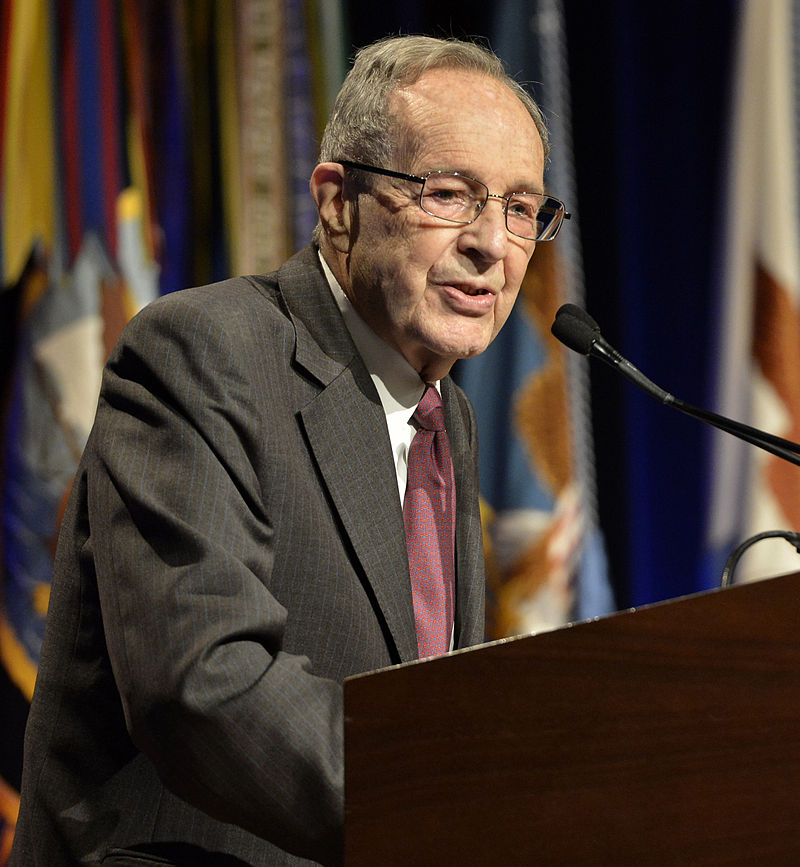
\includegraphics[height=4cm]{images/william-perry.jpg}
			\caption{William J. Perry, 19th Secretary of Defence for the United States under President Bill Clinton. Perry was instrumental in streamlining the US military infrastructure. Which formalised the discipline known as Configuration Management in private sector industries.} \label{fig:william}
		\end{wrapfigure}
	
		It was not until the 1960s that CM became a technical discipline of its own, when the DoD released a series of military standards known as the \emph{``480 series"}. These standards were regularly updated and eventually consolidated into MIL-HDBK-61 in 1991, which contained a series of technical standards supported by standards developing organisations (SDO)(personal communication, \cite{dod-history}) \footnote{A Standards Developing Organisation (SDO) is a body whose primary activities revolve around the improvement and development of technical standards within a given field (\cite{history-standards}).}.
		
		\subsection{Adoption into Industry} \label{sec:adoption}
		SDOs regulated their own industries through a collection of standards publications starting in the late 80s and early 90s. These various issues have evolved into a widely distributed an accepted standard on CM known as \emph{ANSI-EIA-649-1998 (EIA-649)}, a venture helmed by the Electronic Industries Alliance. EIA-649 has provided the base for many specialised CM techniques since the 90s, but EIA-649 describes the five primary functions of CM (\cite{EIA-649}). 
		
		\subsection{Software Configuration Management (SCM)} \label{sec:scm}
		Software Configuration Management evolved from the practices of the late 60s when Professor Leon Pressor wrote a thesis on change and configuration control, whilst working with the DoD. He took the some of the basic concepts of CM, which are discussed in Section \ref{sec:principles}, and revised others into tools and techniques that solve the issues that were occurring during software projects. This created a set of distinct emphases that were separate from the emphases in traditional CM (see Section \ref{sec:scm-alterations}).
		
	\section{The 5 Functions of CM/SCM} \label{sec:principles}
	EIA-649 (see Section \ref{sec:adoption}) outlines 5 functions (sometimes known as disciplines) that should be enforced in both hardware and software projects. Together they establish a standard for managing the development of a project (\cite{mil-hdbk}). 
	
	This section will take a brief look at the 5 traditional functions of CM before looking how they differ in SCM, as detailed by the latest version of EIA-649.
	
		\subsection{CM Planning and Management} \label{sec:planning}
		Each project should have a formal document that outlines, in detail, all process that are required for the project. This should be used as a reference for everyone involved. Such a document will include procedures for:
		\begin{itemize}
			\item personnel
			\item responsibilities and resources
			\item training
			\item administrative meeting guidelines
			\item base lining resources (see Section \ref{sec:identify})
			\item configuration control and configuration status accounting (see Sections \ref{sec:control} and \ref{sec:accounting})
			\item naming conventions
			\item audits and reviews (see Section \ref{sec:audit})
			\item subcontractor/vendor CM requirements
		\end{itemize}
		These processes will be created before development of the project has begun. Any changes to this document during the life-cycle of the project should be avoided, to prevent confusion. But if changes are needed, then a Document Change Notice (DCN) should be issued to all personnel. The details of a DCN can be found within a CM document.
		
		\subsection{Configuration Identification (CI)} \label{sec:identify}
		CI involves defining the system and subsystem architectures through the use of baselines. The procedures for changing any part of the system - how the change is identified, documented and tracked through design, development, testing and delivery - is created during this function. 
		
		\subsection{Configuration Control} \label{sec:control}
		Configuration Control is the evaluation of all change-requests and change-proposals to the project and its documentation; including the process for approving or rejecting the changes.
		
		\subsection{Configuration Status Accounting} \label{sec:accounting}
		Configuration Status Accounting dictate the process for recording and reporting configuration item descriptions and all changes from the original designed baseline.
		
		\subsection{Configuration Verification and Audit} \label{sec:audit}
		The final function of CM is the independent review of hardware and software to ensure that the product meets the established performance requirements outlined at the start of the project.
		
		\subsection{Alterations for Software Configuration Management (SCM)} \label{sec:scm-alterations}
		SCM was created to better suit the challenges posed by Software Projects, as stated in Section \ref{sec:scm}. SCM places a greater emphasis on the need to trace changes in the system with the ability to verify that the delivered software does not exceed the original intent for the program. As a result the four functions for SCM are:
		
		\begin{enumerate}
			\item Configuration Identification (CI)
			\item Configuration Change Control
			\item Configuration Status Accounting
			\item Configuration Audits
		\end{enumerate}
	
		The first three functions of SCM are closely linked to their traditional counterparts, see Sections \ref{sec:identify}, \ref{sec:control} and \ref{sec:accounting} for details about SCM 1, 2 and 3. 
		
		Configuration Audits for SCM are separated into two halves, functional and physical, both of which can occur at either delivery or when a change is implemented. Functional audits look at a configuration item to ensure that it meets both the functional and performance requirements. A physical audit ensures that a configuration item is installed within the wider system in accordance with the system design documentation .
		
		Notice that the CM Planning and Management function of traditional CM has been entirely removed from SCM. That is because Design Document, a Software Engineering practice, covers the majority of the same topics \footnote{A Design Document is a technical guide for Developers to use before, during and after Developing a piece of Software.}(\cite{DesignDocExample}).
		
	\section{Using CM} \label{sec:using}
	In this section we will examine how the functions of CM can be utilised within work and personal projects, touching briefly upon the techniques used to accomplish CM. 
	
		\subsection{In the Office} \label{sec:office}
		Historically configuration management has required a dedicated employee, or team of employees for larger projects, in order to function. Typically they would be known as Administrators. This is still true today for complicated projects carried out by large organisations. Outsourcing is another method in which configuration management can be deployed, where an external companies will handle the administration of a project. Small start up firms will incorporate the task of configuration management into a senior member of the development team. In any case, the tools and techniques used will remain the same (\cite{CM-BestPractices}). 
		
		Each function of CM produces a formal product. The first stage (see Section \ref{sec:planning}) creates a document, much like a design document, that informs individuals how to contribute to a project in a way that allows others to understand what was changed. The Administrator of a project creates this document and will ultimately decide how tasks will be completed. There are a range of tools to assist in this task such as \emph{Chef} (\cite{chef}) or \emph{Puppet} (\cite{puppet}) which take a lot of the burden away from the administrator. 
		
		Functions two through five produce a variety of reports. The creation of these documents is detailed by the CM document produced in the first stage. For example; when developing software in a modern formal setting there are two versions of the project at any given time (in most cases), a \emph{master} copy and a \emph{development} copy. When an edit is created it is tested according to the baselines detailed in CI (see Section \ref{sec:identify}) within the development build. The results of the test are recorded, typically by a tool such as \emph{Codeship} (\cite{codeship}). Assuming the tests pass, a request is made to update the Master copy with the new edits. The industry standard is to use a \emph{GitHub pull request} (\cite{github}) to accomplish and record this, including any last minute edits. Finally at the end of each completed feature a review (or audit) of the project is performed to ensure that the work accomplished is relevant to the original specification. 
		
		The above example shows that by producing reports from CM functions two through five and adhering to the guidelines set out by the CM document (see Section \ref{sec:planning}) the functions of CM will be automatically applied to any project. However, the tools will cited in the example will differ from the tools used in a non-software based project. 
		
		\subsection{At Home} \label{sec:home}
		As discussed in Section \ref{sec:history}, the primary function of CM is to ensure that tasks which affect a project are performed in a near identical manner so that individuals can collaborate with minimal training. In the office this could be a trivial task such as how a testing report is filed, to a critical task as to what testing parameters will be used. 
		
		\begin{wrapfigure}{r}{7cm}
			\centering
			
\includegraphics[height=4cm]{images/shopping-list.jpg}
			\caption{An example shopping list that is a prime example of CM techniques being used in home life (\cite{shopping-list}).} \label{fig:shopping}
		\end{wrapfigure}
	
		But the lessons that are learned from CM in industry can be applied to home life as well. Keeping the cleaning supplies in a certain cupboard, writing groceries on a piece of paper as they are used up and having a filing system for important documents are examples of how CM has infiltrated many homes. The majority of families will not realise that they are using tried and tested CM techniques to improve the efficiency of their households. Is it possible to incorporate CM further into our daily lives?
		
		A lot of CM revolves around lists; to do, in progress, audit, done lists are all common place in CM projects. This is because if we tried to remember everything about a project without the aid of lists we would be lost. This is especially true when executing complicated tasks like engineering a bridge or designing logic to control a function. The same can be said for home life as shopping lists (as seen in Figure \ref{fig:shopping}) are common place but why not have a general \emph{to do list}. Expand that list in to a weekly plan on your calendar (app or physical). It would be foolish to execute an industrial project without a detailed plan, personal lives are no less complicated. 
		
		Another key component of CM is knowing where everything related to a project is. Being able to look quickly located bug and testing reports can save a lot of time. The same can be true for knowing exactly where the bleach or light bulbs are kept in the house. It is not enough to know which cupboard these items may be located in, as you would not expect the bug reports to be left in one general folder, the reports may be kept in a dated folder and the files timestamped with the summary of the issue. So why not have baskets in your cleaning supplied cupboard, each with their own dedicated label. Benjamin Franklin once said \enquote{A place for everything and everything in it's place}, this is very true for keeping an efficient household (\cite{cm-at-home}).  
		
	\section{Embracing CM} \label{sec:embracing}
	We have already discussed what CM is and how it came to be in Sections \ref{sec:history} and \ref{sec:principles}. Section \ref{sec:using} covered how CM is utilised in a project. This section will discuss the benefits of CM and the costs of incorporating it into a project. 
	
		\subsection{Benefits of CM} \label{sec:benefits}
		As stated throughout this paper the principle benefit of CM is that it allows for individuals to contribute to a project without disrupting other contributors with minimal training. Increased efficiency and communication can be experienced within teams, both internally and externally (\cite{unexpected-benefits}). Section \ref{sec:office} states that each function of CM produces a formal product, usually in the form of a report. These reports form a paper trail that records every detail of a project, which in turn can be reviewed to see where the project (and the development methodologies used) can be improved for future use. Products that were built using CM tend to be more reliable due to the higher level of scrutiny that is inherited from the use of CM techniques (\cite{benefits}).
		
		\subsection{Costs} \label{sec:costs}
		CM is not free, there are associated costs with it. Creating the CM document from the first function is a huge undertaking (see Section \ref{sec:planning}). We can either purchase a licence to a tool that will create our CM rules, or hire skilled administrators to write the document from scratch. No matter what we do it will cost both money and time. We may also need additional licences for tools to generate the reports for the other five functions of CM, and administrators to ensure that the CM system is working in an optimal manner. So there is a huge time and cost investment required to get CM off the ground (\cite{costs}). For example; Chef, a popular automated CM tool, has a licence cost of \$137 per node (per computer using Chef) (\cite{chef-pricing}).
		
	\section{Conclusion} \label{sec:conc}
	In this paper we have discussed the origins of Configuration Management (CM), the adoption of CM into industry and the creation of Software Configuration Management (see Section \ref{sec:history}). We gained an understanding of the functions that govern CM (see Section \ref{sec:principles}) and how CM is carried out in daily life, both in the office and at home (see Section \ref{sec:using}), before examining the costs and benefits of CM (see Section \ref{sec:embracing}).
	
	It is well known that CM can benefit the majority of projects, with the noticeable exception of simple tasks, increasing efficiency and management quality.  Many CM techniques, such as lists and consistent filing have managed to be incorporated into home life, the argument can be made for further incorporation of CM into the home (see Section \ref{sec:home}). However, it is the associated costs (as described in Section \ref{sec:costs}) that dictate whether it is beneficial to incorporate CM into a project. This is true for both projects at work or home, and is a question that can only be answered by the project administrators.  
	
	\clearpage
	\bibliographystyle{asgm}
	\bibliography{report}
\end{document}

% EOF Document